\documentclass{article}
\usepackage[utf8]{inputenc}
\usepackage{hyperref}
\usepackage[letterpaper, portrait, margin=1in]{geometry}
\usepackage{enumitem}
\usepackage{amsmath}
\usepackage{booktabs}
\usepackage{graphicx}
\usepackage{float}

\usepackage{hyperref}
\hypersetup{
colorlinks=true,
    linkcolor=black,
    filecolor=black,      
    urlcolor=blue,
    citecolor=black,
}
\usepackage{natbib}

\usepackage{titlesec}
  
\title{Homework 6}
\author{Lin Yang}
\date{\today}
  
\begin{document}
\maketitle  
\section{Python}
~\\
1. Since every vehicle equipped with the technology is significantly less fuel-efficient, I believe it is sharp RD. 

~\\
2. There is obvious evidence of two bunching around the cutoff length = 225. So visual evidence of discontinuity may exist. 

\begin{figure}[ht]
\centering
 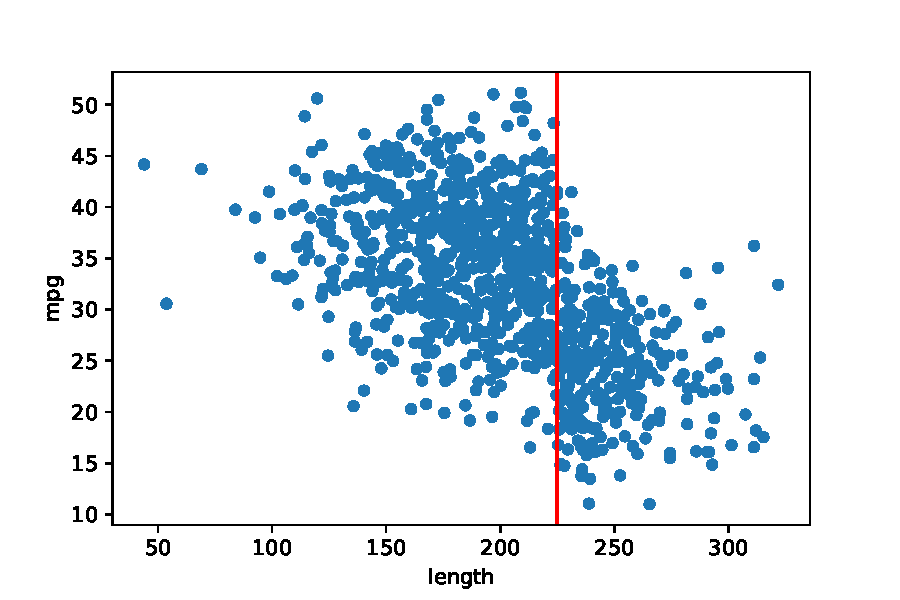
\includegraphics[scale = 0.9]{q2.pdf}
 \caption{Scatter plot of impact of the policy on fuel efficiency}
 
 \end{figure}
 

~\\
3. Fit a first-polynomial to both sides of the cut off in a regression discontinuity design. 
\begin{figure}[H]
\centering
 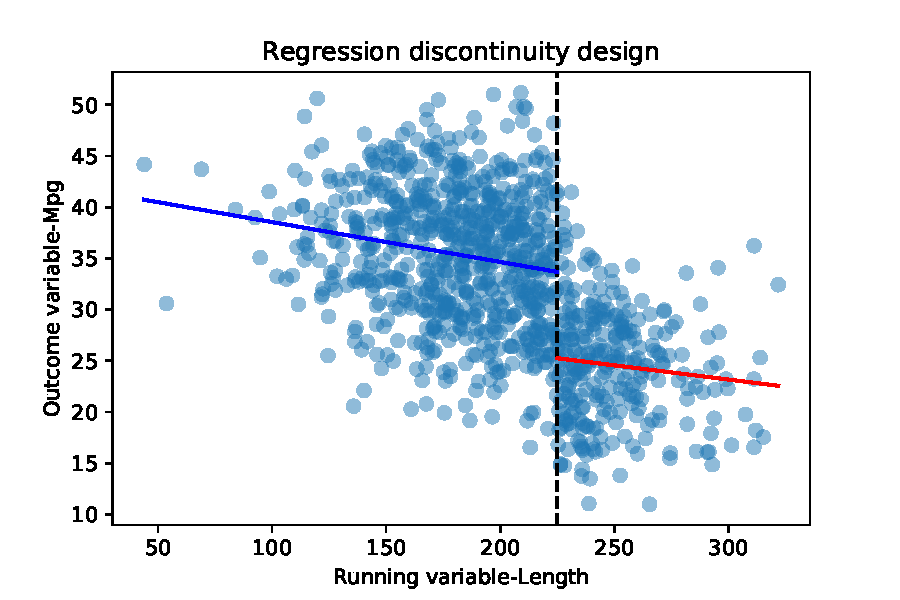
\includegraphics[scale = 0.9]{q3.pdf}
 \caption{Scatter plot of impact of the policy on fuel efficiency and fitted first polynommial}
 
 \end{figure}
The first-stage treatment effect is 0.0111, which is obtained by differencing the estimate (-0.0278) using the points above the cutoff and the estimate (-0.0389) using the points below cutoff and means the mpg for the length above 225 cars is 0.0111 higher than the cars with length less than 225.

~\\
4. Fit a second-polynomial to both sides of the cut off in a regression discontinuity design. 

\begin{figure}[H]
\centering
 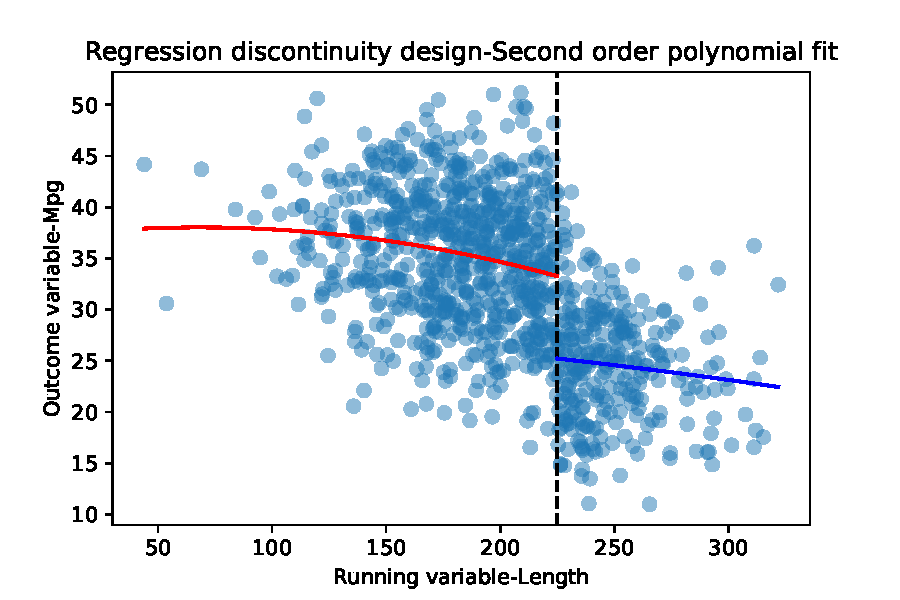
\includegraphics[scale = 0.9]{q4.pdf}
 \caption{Scatter plot of impact of the policy on fuel efficiency and fitted second polynomial}
 
 \end{figure}
 
 The treatment effect estimate is shown in the table below. 
 \begin{table}[H]
 \centering
 \begin{center}
\begin{tabular}{lclc}
\toprule
\textbf{Dep. Variable:}    &       mpg        & \textbf{  R-squared:         } &     0.322   \\
\textbf{Model:}            &       OLS        & \textbf{  Adj. R-squared:    } &     0.321   \\
\textbf{Method:}           &  Least Squares   & \textbf{  F-statistic:       } &     237.2   \\
\textbf{Date:}             & Mon, 27 Feb 2023 & \textbf{  Prob (F-statistic):} &  5.62e-85   \\
\textbf{Time:}             &     23:07:15     & \textbf{  Log-Likelihood:    } &   -3294.2   \\
\textbf{No. Observations:} &        1000      & \textbf{  AIC:               } &     6594.   \\
\textbf{Df Residuals:}     &         997      & \textbf{  BIC:               } &     6609.   \\
\textbf{Df Model:}         &           2      & \textbf{                     } &             \\
\textbf{Covariance Type:}  &    nonrobust     & \textbf{                     } &             \\
\bottomrule
\end{tabular}
\begin{tabular}{lcccccc}
               & \textbf{coef} & \textbf{std err} & \textbf{t} & \textbf{P$> |$t$|$} & \textbf{[0.025} & \textbf{0.975]}  \\
\midrule
\textbf{const} &      35.5552  &        3.239     &    10.978  &         0.000        &       29.199    &       41.911     \\
\textbf{x1}    &       0.0794  &        0.033     &     2.421  &         0.016        &        0.015    &        0.144     \\
\textbf{x2}    &      -0.0005  &     8.14e-05     &    -5.610  &         0.000        &       -0.001    &       -0.000     \\
\bottomrule
\end{tabular}
\begin{tabular}{lclc}
\textbf{Omnibus:}       &  1.918 & \textbf{  Durbin-Watson:     } &    1.536  \\
\textbf{Prob(Omnibus):} &  0.383 & \textbf{  Jarque-Bera (JB):  } &    1.776  \\
\textbf{Skew:}          &  0.008 & \textbf{  Prob(JB):          } &    0.411  \\
\textbf{Kurtosis:}      &  2.794 & \textbf{  Cond. No.          } & 7.05e+05  \\
\bottomrule
\end{tabular}
%\caption{OLS Regression Results}
\end{center}

Notes: \newline
 [1] Standard Errors assume that the covariance matrix of the errors is correctly specified. \newline
 [2] The condition number is large, 7.05e+05. This might indicate that there are \newline
 strong multicollinearity or other numerical problems.
 	
 \end{table}


~\\
5. Fit a fifth-polynomial to both sides of the cut off in a regression discontinuity design. 
\begin{figure}[H]
\centering
 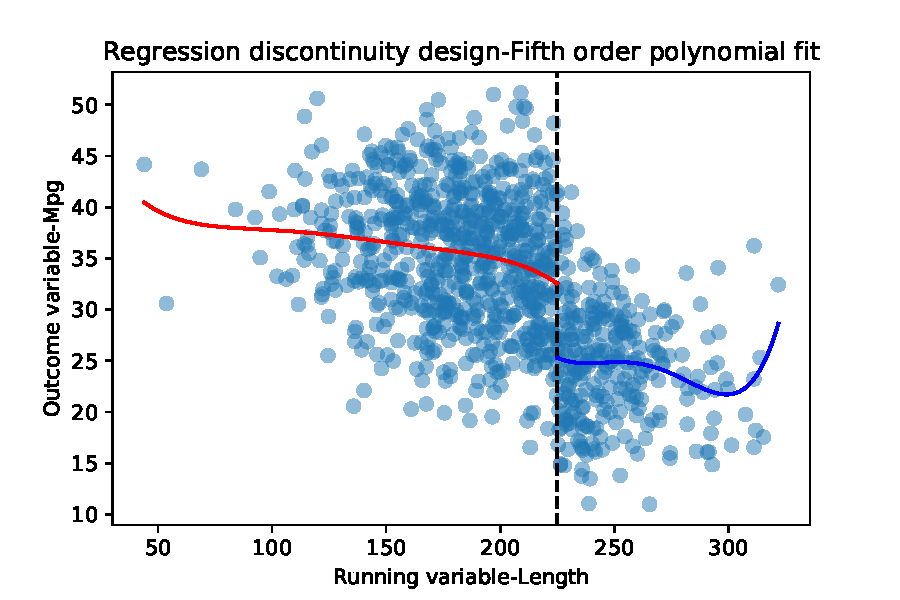
\includegraphics[scale = 0.9]{q5.pdf}
 \caption{Scatter plot of impact of the policy on fuel efficiency and fitted fifth polynomial}
 
 \end{figure}


 The treatment effect estimate is shown in the table below. 
 \begin{table}[H]
 \centering
 \begin{center}
\begin{tabular}{lclc}
\toprule
\textbf{Dep. Variable:}    &       mpg        & \textbf{  R-squared:         } &     0.356   \\
\textbf{Model:}            &       OLS        & \textbf{  Adj. R-squared:    } &     0.352   \\
\textbf{Method:}           &  Least Squares   & \textbf{  F-statistic:       } &     109.7   \\
\textbf{Date:}             & Mon, 27 Feb 2023 & \textbf{  Prob (F-statistic):} &  2.63e-92   \\
\textbf{Time:}             &     23:12:18     & \textbf{  Log-Likelihood:    } &   -3269.2   \\
\textbf{No. Observations:} &        1000      & \textbf{  AIC:               } &     6550.   \\
\textbf{Df Residuals:}     &         994      & \textbf{  BIC:               } &     6580.   \\
\textbf{Df Model:}         &           5      & \textbf{                     } &             \\
\textbf{Covariance Type:}  &    nonrobust     & \textbf{                     } &             \\
\bottomrule
\end{tabular}
\begin{tabular}{lcccccc}
               & \textbf{coef} & \textbf{std err} & \textbf{t} & \textbf{P$> |$t$|$} & \textbf{[0.025} & \textbf{0.975]}  \\
\midrule
\textbf{const} &      59.8980  &       26.869     &     2.229  &         0.026        &        7.171    &      112.625     \\
\textbf{x1}    &      -0.5413  &        0.897     &    -0.603  &         0.546        &       -2.302    &        1.219     \\
\textbf{x2}    &       0.0033  &        0.011     &     0.294  &         0.769        &       -0.019    &        0.025     \\
\textbf{x3}    &    5.578e-06  &     6.59e-05     &     0.085  &         0.933        &       -0.000    &        0.000     \\
\textbf{x4}    &   -9.699e-08  &     1.84e-07     &    -0.528  &         0.598        &    -4.58e-07    &     2.64e-07     \\
\textbf{x5}    &    1.905e-10  &     1.96e-10     &     0.971  &         0.332        &    -1.94e-10    &     5.75e-10     \\
\bottomrule
\end{tabular}
\begin{tabular}{lclc}
\textbf{Omnibus:}       &  4.956 & \textbf{  Durbin-Watson:     } &    1.501  \\
\textbf{Prob(Omnibus):} &  0.084 & \textbf{  Jarque-Bera (JB):  } &    4.140  \\
\textbf{Skew:}          & -0.069 & \textbf{  Prob(JB):          } &    0.126  \\
\textbf{Kurtosis:}      &  2.717 & \textbf{  Cond. No.          } & 8.97e+13  \\
\bottomrule
\end{tabular}
%\caption{OLS Regression Results}
\end{center}

Notes: \newline
 [1] Standard Errors assume that the covariance matrix of the errors is correctly specified. \newline
 [2] The condition number is large, 8.97e+13. This might indicate that there are \newline
 strong multicollinearity or other numerical problems.
 	
 \end{table}
~\\
6. Using the discontinuity as an instrument for miles per gallon, estimate the impact of mpg on the vehicle's sale price using 2sls by hand. 
Results from the second stage is shown in table below. 
\begin{table}[H]
	\centering
	\begin{center}
\begin{tabular}{lclc}
\toprule
\textbf{Dep. Variable:}    &      price       & \textbf{  R-squared:         } &     0.220   \\
\textbf{Model:}            &       OLS        & \textbf{  Adj. R-squared:    } &     0.219   \\
\textbf{Method:}           &  Least Squares   & \textbf{  F-statistic:       } &     140.9   \\
\textbf{Date:}             & Sun, 26 Feb 2023 & \textbf{  Prob (F-statistic):} &  1.32e-54   \\
\textbf{Time:}             &     23:13:02     & \textbf{  Log-Likelihood:    } &   -9557.3   \\
\textbf{No. Observations:} &        1000      & \textbf{  AIC:               } & 1.912e+04   \\
\textbf{Df Residuals:}     &         997      & \textbf{  BIC:               } & 1.914e+04   \\
\textbf{Df Model:}         &           2      & \textbf{                     } &             \\
\textbf{Covariance Type:}  &    nonrobust     & \textbf{                     } &             \\
\bottomrule
\end{tabular}
\begin{tabular}{lcccccc}
                      & \textbf{coef} & \textbf{std err} & \textbf{t} & \textbf{P$> |$t$|$} & \textbf{[0.025} & \textbf{0.975]}  \\
\midrule
\textbf{Intercept}    &    1.741e+04  &      747.885     &    23.275  &         0.000        &     1.59e+04    &     1.89e+04     \\
\textbf{predictedmpg} &     158.2799  &       26.029     &     6.081  &         0.000        &      107.201    &      209.359     \\
\textbf{car}          &   -4743.0637  &      310.432     &   -15.279  &         0.000        &    -5352.238    &    -4133.889     \\
\bottomrule
\end{tabular}
\begin{tabular}{lclc}
\textbf{Omnibus:}       &  4.452 & \textbf{  Durbin-Watson:     } &    1.986  \\
\textbf{Prob(Omnibus):} &  0.108 & \textbf{  Jarque-Bera (JB):  } &    4.538  \\
\textbf{Skew:}          &  0.112 & \textbf{  Prob(JB):          } &    0.103  \\
\textbf{Kurtosis:}      &  3.242 & \textbf{  Cond. No.          } &     235.  \\
\bottomrule
\end{tabular}
%\caption{OLS Regression Results}
\end{center}

Notes: \newline
 [1] Standard Errors assume that the covariance matrix of the errors is correctly specified.
\end{table}

\section{Stata}
~\\
1. (a) The average treatment effect of mpg on price is 135.41. 

\begin{table}[H]
	\centering
	\input{Stata1.tex}
\end{table}
~\\

(b) 
\begin{figure}[H]
\centering
 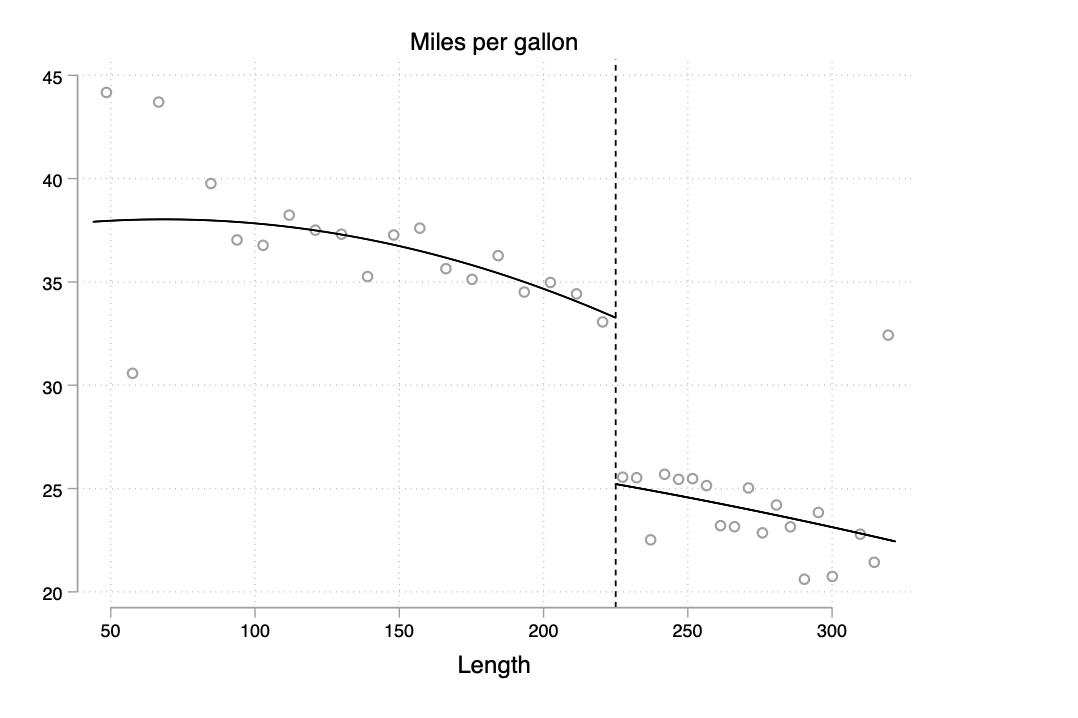
\includegraphics[scale = 0.9]{stata1b.png}
 \caption{Scatter plot of impact of the policy on fuel efficiency and fitted second polynomial}
 
 \end{figure}
 
 ~\\
 2. Yes. I think it is a valid instrument. 

\end{document}
